
%*******************************************************************************
%*********************************** Conclusions ***************************
%*******************************************************************************
%!TEX root = 0.main.tex

\section{Conclusions}\label{sec:Chapter4}




\subsection{Experimental validation: SHREC17}
\label{sec:Chapter5:Experimental validation}
Gusset et al. \cite{Gusset} implemented the graph proposed in this work in a GCNN and three other rotation equivariant neural networks on a popular classification problem \cite{SHREC17}. The four models tested were the following: the original version of DeepSphere, Deepsphere \textit{Optimal} - obtained implementing the thresholding procedure described in this work in section \ref{sec:Chapter2:How to build a good graph} - and the traditional SCNNs of Cohen et al. \cite{SCNN} introduced in section \ref{sec:Chapter1:SCNN} and of Esteves et al. \cite{Esteves}
\paragraph{On the Equiangular sampling}. They compare with two different metrics  (accuracy, F1-score) the performances of these four rotation invariant models, while also comparing the speed of inference and of training of each model. Results are shown in table \ref{tab:SHREC17_class}.  It can be seen how \textit{DeepSphere Optimal} has \textit{always} the highest score between all the rotation equivariant models, no matter the evaluation metric. Furthermore, its performances in terms of speed of inference and training are second only to DeepSphere, remaining by far faster than the other two SCNNs. 
\begin{table}[ht]
	\centering
	\begin{tabular}{l|c c r r r}
		\multicolumn{1}{l}{} & \multicolumn{2}{c}{performance} & \multicolumn{1}{c}{size} & \multicolumn{2}{c}{speed}\\
		\cmidrule(lr){2-3} \cmidrule(lr){4-4} \cmidrule(lr){5-6}
		\multicolumn{1}{l}{Method} & Accuracy & F1-score & params & inference & training \\ \hline
		Cohen \emph{s2cnn\_simple} & 78.59 & 78.85 & 400k & 12ms & 32h\\
		Esteves \emph{sphericalcnn} & 79.18 & 79.36 & 500k & 9.8ms & 2h52\\ \hline
		Deepsphere & 73.36 & 73.67 & 190k & \textbf{0.98ms} & \textbf{43m} \\
		\textbf{Deepsphere \emph{Optimal}} & \textbf{80.42} & \textbf{80.65} & 190k & 1.0ms & 48m
	\end{tabular}
	\caption{Results form \cite{Gusset}. Performances of four rotation equivariant GCNNs and two SCNNs on the popular classification task SHREC17.}
	\label{tab:SHREC17_class}
\end{table}
\paragraph{On HEALPix }
Gusset et al. repeated the same test on the same dataset on a HEALPix sampling with $N_{side}=32$. Results can be seen in table \ref{table:results}.
\begin{table}[h!]
	\centering
	\begin{tabular}{ c|c|c } 
		& DeepSphere & DeepSphere \textit{Optimal} \\ 
		\hline
		accuracy & 82.23\% & 82.76\% \\ 
	\end{tabular}
	\caption{\label{table:results}Results form Gusset et al. Accuracy on the HEALPix sampling}
\end{table}
Being the new graph of DeepSphere Optimal more equivariant to rotations, we expected to see an improvement in the accuracy, as we did in the equiangular case. The fact that this improvement was not observed on HEALPix means that, in this case, the original DeepSphere graph $W$ \textit{is already sufficiently equivariant to rotations}. By this we mean that for this task, being equivariant to rotations of the low frequency eigenmodes is sufficient to obtain good results, and that being rotation equivariant to the higher frequencies does not lead to any improvement.

\subsection{Confront of different Discrete Laplacians on the equiangular sampling}
We conclude by showing how the different discrete Laplacians $\mathbf L$ illustrated so far compare in terms of equivariance error and computational time of the filter $\mathcal F(\mathbf f) = \mathbf L\mathbf f$. We can see how the three sparse discrete Laplacians are one order of magnitude faster than the two full Laplacians. The FEM approach is actually able to reduce the equivariance error compared to the HKGL, and it stays low even when using the sparse, lumped approximation $B^{-1}A$. The lumped FEM Laplacian $D^{-1}A$ performs really well, and gets close to the performances of the graph Laplacian of Khasanova and Frossard. 
\begin{figure}[h!]
	\centering
	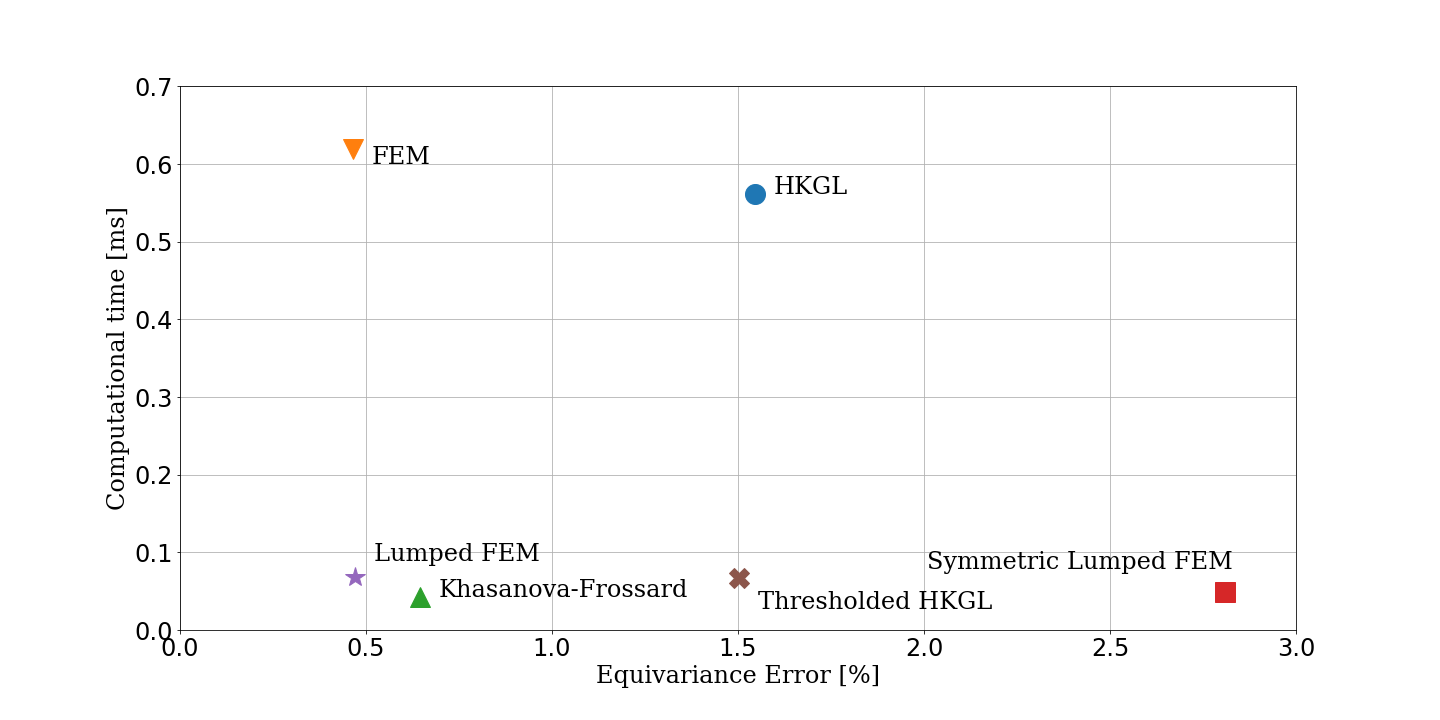
\includegraphics[width=\textwidth]{../codes/06.Equivariance_error/tradeoff.png}
	\caption{\label{fig:tradeoff}Trade-off between computational time and equivariance error for the filter $\mathbf L$ for different discrete Laplacians on the equiangular sampling}
\end{figure}

\subsection{Final considerations and future work}


Having a metric means using a \textit{non-symmetric matrix} $B^{-1}A$ such that the generalized eigenvalue problem $Av = \lambda B v$ is such that $v_i$ approximates the corresponding sampled SH and $VBV^T=I$. With a graph this is not possible since we restrict ourself to \textit{symmetric} Laplacians and thus make it impossible to incorporate a metric $B$, since the symmetry of $L$ imposes $VV^T=I$. However, there are good approximations that even by being symmetric perform well: the Khasanova-Frossard graph is an example. Further research would be 